%%%%%%%%%%%%%%%%%%%%%%%%%%%%%%%%%%%%%%
% Multiplicative domain poster
% Created by Nathaniel Johnston
% August 2009
% http://www.nathanieljohnston.com/2009/08/latex-poster-template/
%%%%%%%%%%%%%%%%%%%%%%%%%%%%%%%%%%%%%%

\documentclass[final]{beamer}
\usepackage[scale=1.24]{beamerposter}
\usepackage{graphicx}			% allows us to import images

%-----------------------------------------------------------
% Custom commands that I use frequently
%-----------------------------------------------------------

\newcommand{\bb}[1]{\mathbb{#1}}
\newcommand{\cl}[1]{\mathcal{#1}}
\newcommand{\fA}{\mathfrak{A}}
\newcommand{\fB}{\mathfrak{B}}
\newcommand{\Tr}{{\rm Tr}}
\newtheorem{thm}{Theorem}

%-----------------------------------------------------------
% Define the column width and poster size
% To set effective sepwid, onecolwid and twocolwid values, first choose how many columns you want and how much separation you want between columns
% The separation I chose is 0.024 and I want 4 columns
% Then set onecolwid to be (1-(4+1)*0.024)/4 = 0.22
% Set twocolwid to be 2*onecolwid + sepwid = 0.464
%-----------------------------------------------------------

\newlength{\sepwid}
\newlength{\onecolwid}
\newlength{\twocolwid}
\setlength{\paperwidth}{48in}
\setlength{\paperheight}{36in}
\setlength{\sepwid}{0.024\paperwidth}
\setlength{\onecolwid}{0.22\paperwidth}
\setlength{\twocolwid}{0.464\paperwidth}
\setlength{\topmargin}{-0.5in}
\usetheme{confposter}
\usepackage{exscale}

%-----------------------------------------------------------
% The next part fixes a problem with figure numbering. Thanks Nishan!
% When including a figure in your poster, be sure that the commands are typed in the following order:
% \begin{figure}
% \includegraphics[...]{...}
% \caption{...}
% \end{figure}
% That is, put the \caption after the \includegraphics
%-----------------------------------------------------------

\usecaptiontemplate{
\small
\structure{\insertcaptionname~\insertcaptionnumber:}
\insertcaption}

%-----------------------------------------------------------
% Define colours (see beamerthemeconfposter.sty to change these colour definitions)
%-----------------------------------------------------------

\setbeamercolor{block title}{fg=ngreen,bg=white}
\setbeamercolor{block body}{fg=black,bg=white}
\setbeamercolor{block alerted title}{fg=white,bg=dblue!70}
\setbeamercolor{block alerted body}{fg=black,bg=dblue!10}

%-----------------------------------------------------------
% Name and authors of poster/paper/research
%-----------------------------------------------------------

\title{Spectral Stability of Multi-Pulse Solutions to the Suspension Bridge Equation}
\author{Ross Parker, Todd Kapitula, Bj\"{o}rn Sandstede}
\institute{Division of Applied Mathematics, Brown University}

%-----------------------------------------------------------
% Start the poster itself
%-----------------------------------------------------------
% The \rmfamily command is used frequently throughout the poster to force a serif font to be used for the body text
% Serif font is better for small text, sans-serif font is better for headers (for readability reasons)
%-----------------------------------------------------------

\begin{document}
\begin{frame}[t]
  \begin{columns}[t]												% the [t] option aligns the column's content at the top
    \begin{column}{\sepwid}\end{column}			% empty spacer column

% first column
    \begin{column}{\onecolwid}
     
      \begin{block}{Suspension Bridge Equation}
        \rmfamily{
          Original model for waves on a suspended beam
            \[ u_{tt} + u_{xxxx} + u^+ - 1 = 0 \]
          Smooth approximation to this model
            \[ u_{tt} + u_{xxxx} + e^{u} - 1 = 0 \]
          In a co-moving frame with speed $c$
            \[ u_{tt} - 2 c u_{x t} + u_{xxxx} + c^2 u_{xx} + e^{u} - 1 = 0 \]
        }
      \end{block}

      \begin{block}{Homoclinic Orbits}
        \rmfamily{
          Equilibrium solution satisfies ODE
            \begin{equation}\label{eqODE}
             u_{xxxx} + c^2 u_{xx} + e^{u} - 1 = 0
             \end{equation}
          For $c \in (0, \sqrt{2})$, eigenvalues of linearization about 0 are
          \vskip0.1ex
            \[ \mu = \pm \sqrt{\frac{-c^2 \pm \sqrt{c^4 - 4}}{2} } = \pm \alpha \pm \beta i,\]
          \vskip1ex
            2D stable manifold, 2D unstable manifold\\
          \vskip1ex
          \textbf{Theorem 1. }(VdB) For $c^2 \in [0.5, 1.9]$, a homoclinic orbit (single pulse) solution $q(x; c)$ exists which is smooth, even, and decays exponentially to 0 as $x \rightarrow \pm \infty.$
        }
      \end{block}

      \vskip1ex

      \begin{block}{Numerical Construction}
        \rmfamily{

          Primary pulse solutions constructed numerically using the string method [Chamard2011].

          \begin{figure}
          \begin{center}
          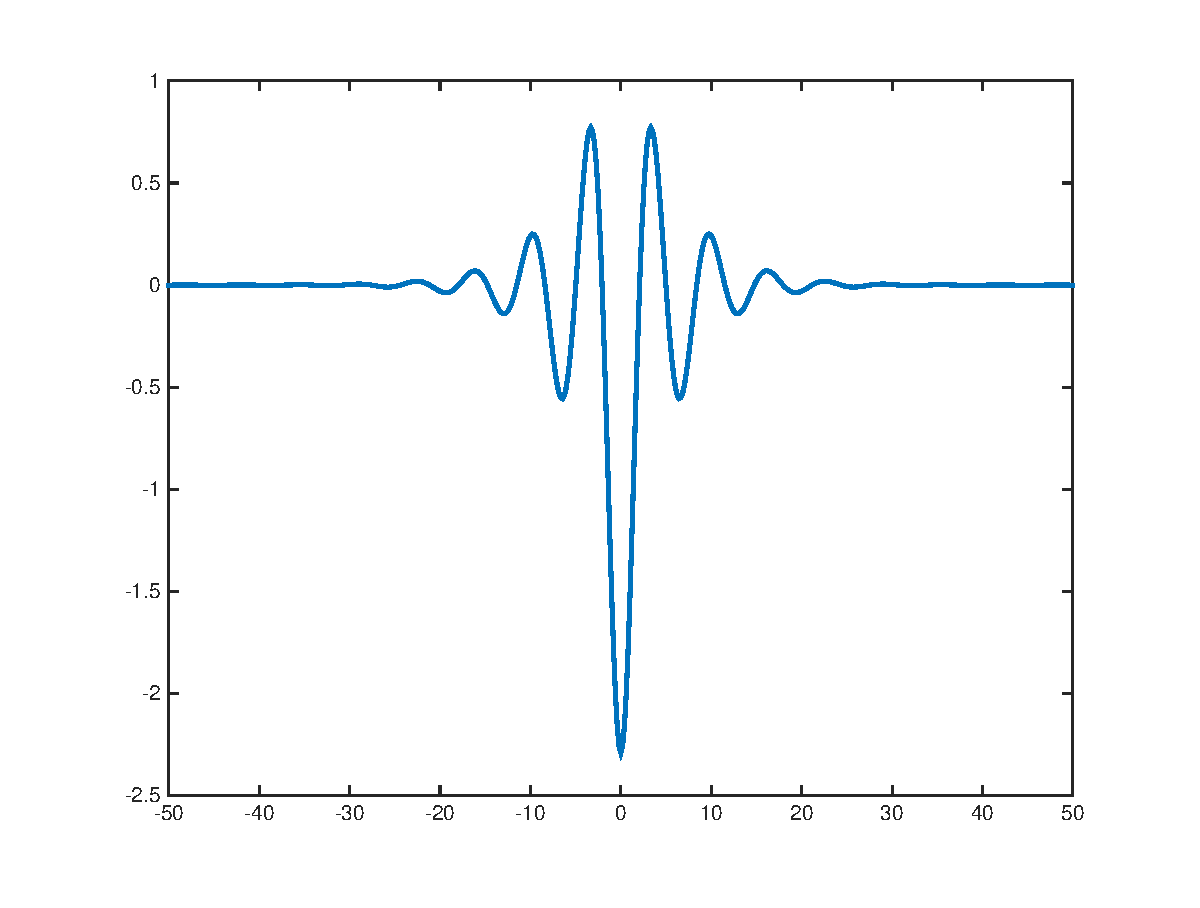
\includegraphics[width=13cm]{images/single1354.eps}
          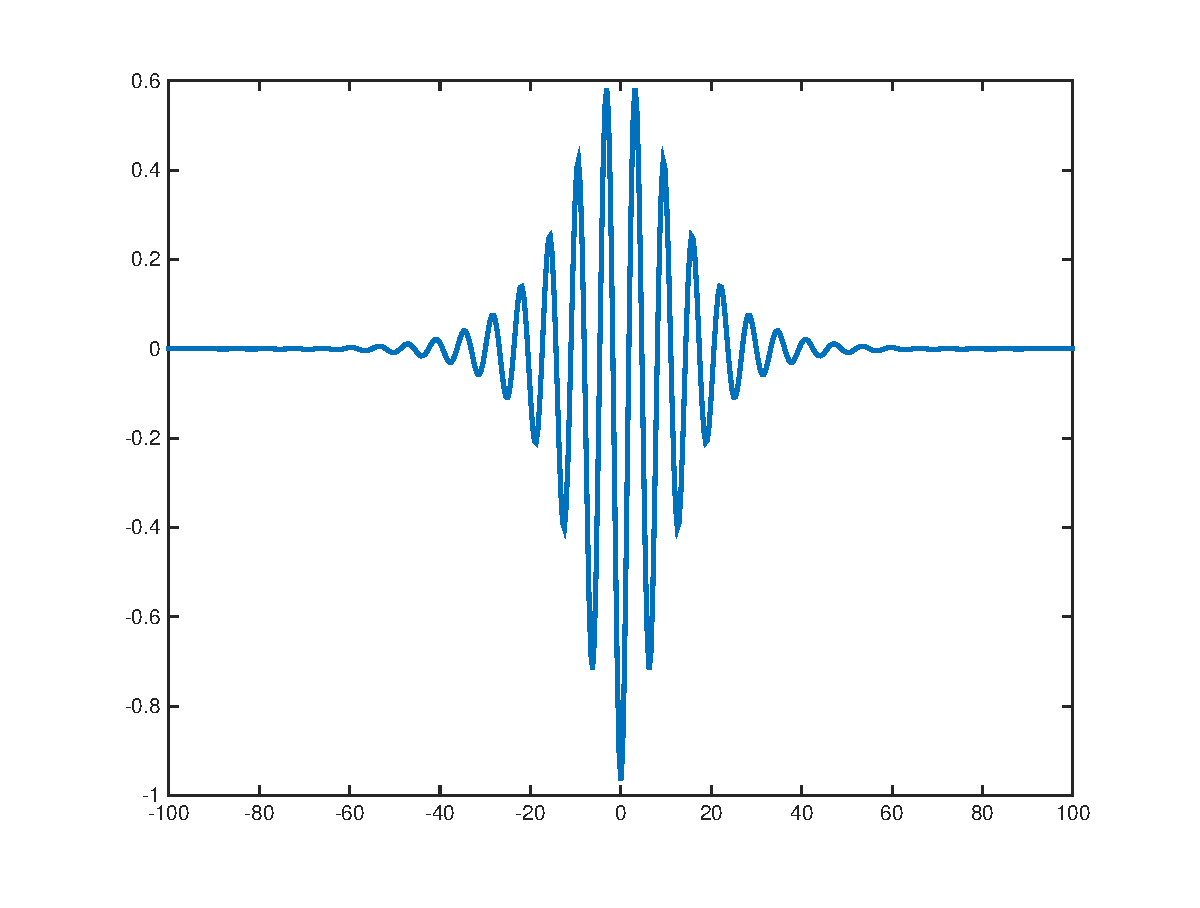
\includegraphics[width=13cm]{images/single14.eps}
          \caption{Primary pulse solutions, $c = 1.354$ (left) and $c = 1.40$ (right).}
          \label{fig:single1}
          \end{center}
          \end{figure}
        }
      \end{block}
 
    \end{column}

\begin{column}{\sepwid}\end{column}     % empty spacer column

% second column
    \begin{column}{\onecolwid}

      \begin{block}{Multi-Pulse Solutions}
      \rmfamily{
      \textbf{Theorem 2. }(San97) Let $q(x; c)$ be a localized homoclinic orbit solution to \eqref{eqODE}. Choose any integer $n \geq 2$ and any sequence of nonnegative integers $k_1, \dots, k_{n-1}$ such that at least one of the $k_j \in \{0, 1 \}$. Then

      \begin{itemize}
        \item For any sufficiently large integer $m$, there exists a unique $n-$modal solution $q_n(x, c)$ to \eqref{eqODE} This solution resembles $n$ well-separated copies of the primary pulse $q(x; c)$. The distance between successive peaks is given by the $X_1, \dots, X_{n-1}$, where
        \begin{equation*}
        X_j \approx \frac{\pi}{\beta}(2 m + k_j) + C
        \end{equation*}

        \item Linearization of \eqref{eqODE} about the $n-$pulse $q_n(x; c)$ is given by

          \begin{equation}\label{defA0}
          A_0(q_n) = \partial_x^4 + c^2 \partial_x^2 + e^{q_n}.
          \end{equation} 

          $A_0(q_n)$ has precisely $n$ real eigenvalues $\nu_j$ close to 0, where $\nu_n = 0$ is a simple eigenvalue, and for $j = 1, \dots, n-1$,

          \begin{align*}
          \nu_j < 0 \text{ if } k_j \text{ is odd} \\
          \nu_j > 0 \text{ if } k_j \text{ is even} 
          \end{align*}

        \end{itemize}

        \begin{figure}
        \begin{center}
        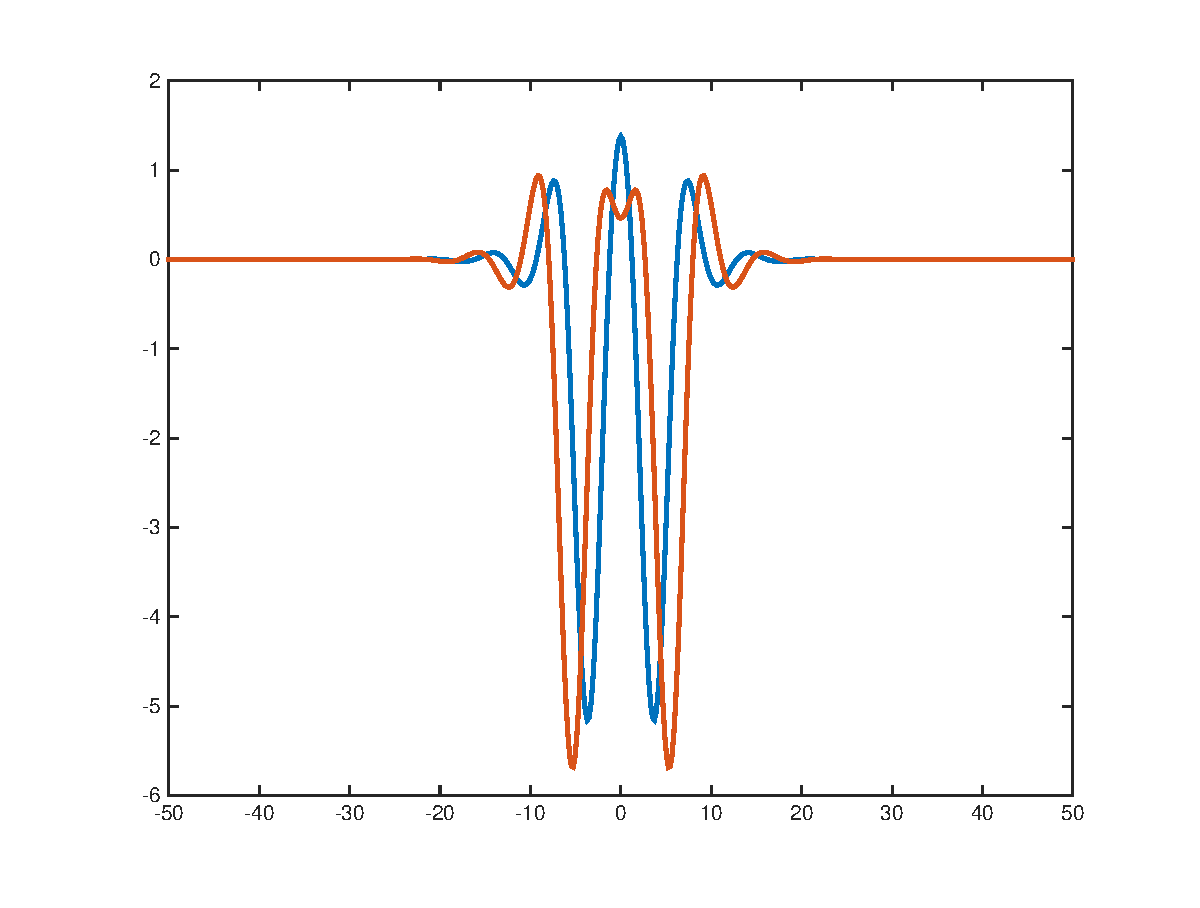
\includegraphics[width=13cm]{images/double12_12.eps}
        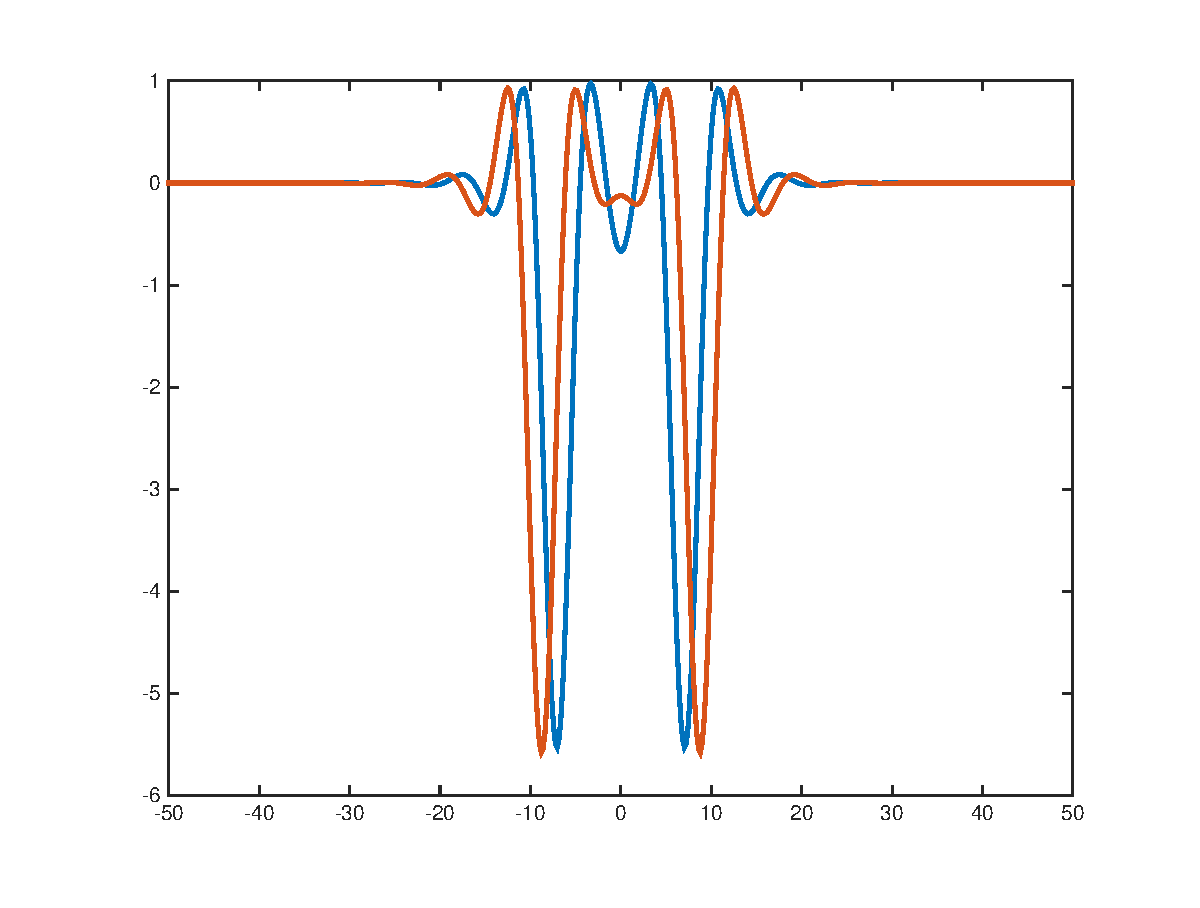
\includegraphics[width=13cm]{images/double12_34.eps}
        \caption{First four 2-pulse solutions to \eqref{eqODE}, $c = 1.2$}
        \label{fig:double}
        \end{center}
        \end{figure}
      }
      \end{block} 

      \vskip1ex

      \begin{block}{PDE Eigenvalue Problem}
      \rmfamily{
      Linearization of the PDE \eqref{suspc} about the $n-$pulse $q_n(x; c)$ is the quadratic eigenvalue problem

      \begin{equation}\label{quadeig}
      P_2(\lambda; q_n)v =  [A_2 \lambda^2 + A_1 \lambda + A_0(q_n)]v = 0,
      \end{equation}

      where $A_0(q_n)$ is defined in \eqref{defA0} and 

      \begin{align}
      A_1 &= -2 c \partial_x \\
      A_2 &= I
      \end{align}

      }
      \end{block}

    \end{column}

\begin{column}{\sepwid}\end{column}     % empty spacer column

% third column
    \begin{column}{\onecolwid}
      \begin{block}{Essential Spectrum}
        \rmfamily{
          The essential spectrum of \eqref{quadeig} is purely imaginary and is bounded away from the origin.

        }
      \end{block}

      \begin{block}{Krein Matrix, Definition}
        \rmfamily{
        Consider a polynomial eigenvalue of the form
        \begin{equation}
        P_n(\lambda) = \sum_{j=0}^n \lambda_j A_j
        \end{equation}
        where the operators $A_j$ are Hermitian for $j$ even and skew-Hermitian for $j$ odd.
        \vskip1ex
        The Krein Matrix is a matrix-valued function $K(\lambda)$ with the properties that for $\lambda \in i\mathbb{R}$
        \begin{itemize}
          \item $K(\lambda)$ is meromorphic.
          \item $\det K(\lambda) = 0$ only if $\lambda$ is a polynomial eigenvalue.
          \item $K(\lambda)$ can be used to determine the Krein signature of a polynomial eigenvalue.
        \end{itemize}
        }
      \end{block}

      \vskip1ex

      \begin{block}{Krein Matrix, Construction}
      \rmfamily{
      \begin{itemize}
        \item Let $S$ be the $n-$dimensional space 

        \begin{equation}\label{defS}
        S = \text{span}\{s_1, \dots, s_n \},
        \end{equation}

        where $s_j(x)$ are the eigenfunctions corresponding to the small eigenvalues $\nu_j$, which are defined in Theorem 2. 

        \item The operator $A_0(q_n)$ is boundedly invertible on $S^\perp$.

        \item The Krein matrix is defined by

        \begin{equation}\label{Kreinmatrix}
        [K_S(z)]_{jk} = 
        \langle s_j , P_2(iz)s_k\rangle 
        - \langle s_j , P_2(iz) P_{S^{\perp}} (P_{S^{\perp}} P_2(iz)|_{S^{\perp}} )^{-1} P_{S^{\perp}} P_2(iz) s_k \rangle
        \end{equation}

      \end{itemize}
      }
      \end{block}

    \end{column}

  \begin{column}{\sepwid}\end{column}			% empty spacer column

  \begin{column}{\onecolwid}

    \begin{block}{Future Work}
        \rmfamily{
        \begin{itemize}
          \item Prove that the eigenvalues of the potentially stable double pulse are pure imaginary to leading order in the pulse distance
          \item Prove spectral stability for the periodic case
          \item Examine stability of multipulse solutions for lattice PDEs
        \end{itemize}
        }
      \end{block} 

    \vskip1ex
  
    \begin{block}{References}
      \small{\rmfamily{\begin{thebibliography}{99}
      \bibitem{Buf}Buffoni B and S\'er\'e E. \emph{A global condition for quasi-random behaviour in a class of conservative systems}. Commun. Pure Appl. Math., 49 (1996), 285-305.
      \bibitem{Chug}Chugunova M and Pelinovsky P. \emph{Two-pulse solutions in the fifth-order KdV equation: Rigorous theory and numerical approximations}. Discrete and Continuous Dynamical Systems, Series B 8.4 (2007), 773-800.
      \bibitem{Grov}Groves M D. \emph{Solitary-wave solutions to a class of fifth-order model equations}. Nonlinearity, 11 (1998), 341-353.
      \bibitem{Sand} Sandstede B. \emph{Stability of multiple-pulse solutions}. Trans. Am. Math. Soc., 350 (1998), 429-472.
      \end{thebibliography}}}
    \end{block}

    \vskip1ex

    \begin{block}{Acknowledgments}
      \small{\rmfamily{This work is supported by the NSF Grant 1148284 }} \\
      \vspace{0.5in}
    \end{block}
  \end{column}
  \begin{column}{\sepwid}\end{column}			% empty spacer column
 \end{columns}
\end{frame}
\end{document}
